\section{Sezione Introduttiva}

\subsection{Team Members}
I membri del gruppo sono:
\begin{itemize}
    \item Giulio Gualtiero, 234656, GitHub: \href{https://github.com/GiulioGualtiero}{GiulioGualtiero}
    \item Jago Revrenna, 235081, GitHub: \href{https://github.com/jagorev}{jagorev}
    \item Tommaso Onori, 234893, GitHub: \href{https://github.com/TommasoOnori}{TommasoOnori}
\end{itemize}

\subsection{Project Idea}
Il progetto prevede lo sviluppo di un sistema intelligente per la gestione dei rifiuti a Trento, composto da un'app mobile per i cittadini e una web app per il Comune. L'obiettivo è ottimizzare la raccolta e lo smaltimento tramite notifiche, segnalazioni e monitoraggio in tempo reale, migliorando l'efficienza e la sostenibilità del servizio.
\subsection{External References}
Collegamenti a risorse esterne:
\begin{itemize}
    \item Repository GitHub: \href{https://github.com/jagorev/EcoTrack}{EcoTrack}
    \item Swagger HUB: \href{ https://app.swaggerhub.com/apis-docs/universityoftrento/EcoTrackAPI/1.0.0#/}{EcoTrack}
\end{itemize}

\section{Sezione Generale}
\subsection{Strategia di Branching}
Abbiamo scelto il \textbf{Feature Branch Workflow} come strategia di branching poiché, essendo il nostro team composto da soli tre membri, risulta semplice ed efficace: ci consente di lavorare in parallelo su funzionalità diverse senza dover affrontare continuamente conflitti di merge. \\Nel caso del nostro progetto, questo approccio ci aiuta a mantenere il branch master stabile e sempre pronto per l’integrazione, rendendo allo stesso tempo più semplice la gestione e la revisione del codice attraverso pull request pulite e dettagliate per ogni nuova funzionalità o correzione di bug. 
\\Inoltre, tale approccio può essere facilmente integrato, all’occorrenza, con una strategia più strutturata come il \textbf{Gitflow Workflow}, qualora il progetto dovesse crescere in complessità.

\subsection{Product Backlog}
È possibile visualizzare il product backlog di EcoTrack al seguente link: \href{https://docs.google.com/spreadsheets/d/124BGyj-mUSipfd_NPPftBozjqdOnjI-apbYR-fjCgLY/edit?usp=sharing}{EcoTrack - Product Backlog}.
\begin{figure}[H]
    \centering
    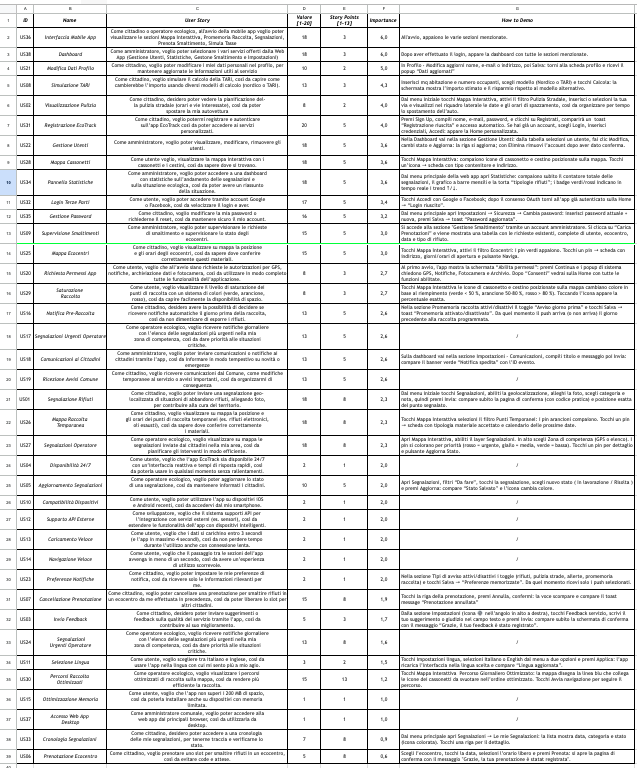
\includegraphics[width=1\linewidth]{D3-G1//Img/Screenshot Product Backlog.png}
    \caption{Product Backlog Overview}
    \label{fig:enter-label}
\end{figure}

\subsection{Definition of Done}
\begin{longtable}{p{3cm}p{11cm}}
\toprule
Categoria & Criterio \\
\midrule
\endfirsthead
\toprule
Categoria & Criterio \\
\midrule
\endhead
Qualità del Codice & Codice conforme agli standard di stile. Nessun errore dev'essere presente. \\
Test e Validazione & Validazione su ambiente di sviluppo o staging completata. \\
Documentazione & Documentazione tecnica aggiornata. Commenti chiari all'interno del codice dove necessario. \\
Sicurezza & Gestione sicura dei dati utente e delle credenziali. \\
Revisione & Code review completata e approvata da almeno un altro membro del team. Correzione di tutte le osservazioni emerse. \\
Deployabilità & Funzionalità integrabile nel ramo principale senza conflitti. Pronta per la release successiva o incremento sprint. \\
\bottomrule
\end{longtable}

\section{Sezione Sprint}
\subsection{Obiettivo dello Sprint}
L’obiettivo del primo sprint è quello di \textbf{realizzare una prima versione funzionante dell’applicazione EcoTrack}, che costituisca una base solida su cui sviluppare le funzionalità successive. \\In questo sprint, il team si concentrerà sullo \textbf{sviluppo delle funzionalità core}, selezionate tra le 15 user stories più importanti.
\\Lo scopo non è quello di rilasciare un prodotto completo in tutte le sue parti, ma una app già utilizzabile nelle sue funzioni essenziali.

\subsection{Sprint Planning}
\subsubsection{Sprint Backlog}
È possibile visualizzare il primo sprint backlog di EcoTrack al seguente link: \href{https://docs.google.com/spreadsheets/d/1UHLnqPdF-jQ3u2Tjfu37wLQoLWdG6EZI/edit?usp=sharing&ouid=117231945359659980757&rtpof=true&sd=true}{EcoTrack - Sprint Backlog}.
\begin{figure}[H]
    \centering
    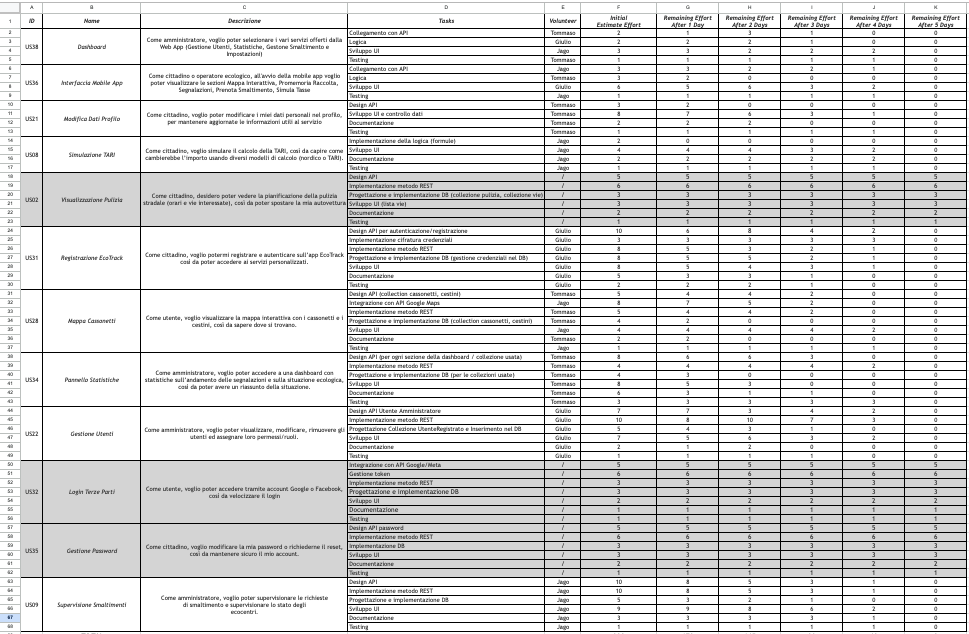
\includegraphics[width=1\linewidth]{D3-G1//Img/Screenshot Sprint.png}
    \caption{Sprint Backlog Overview. Le user stories evidenziate in grigio non sono state implementate.}
    \label{fig:enter-label}
\end{figure}

\subsubsection{Burndown Chart}
\begin{figure}[H]
    \centering
    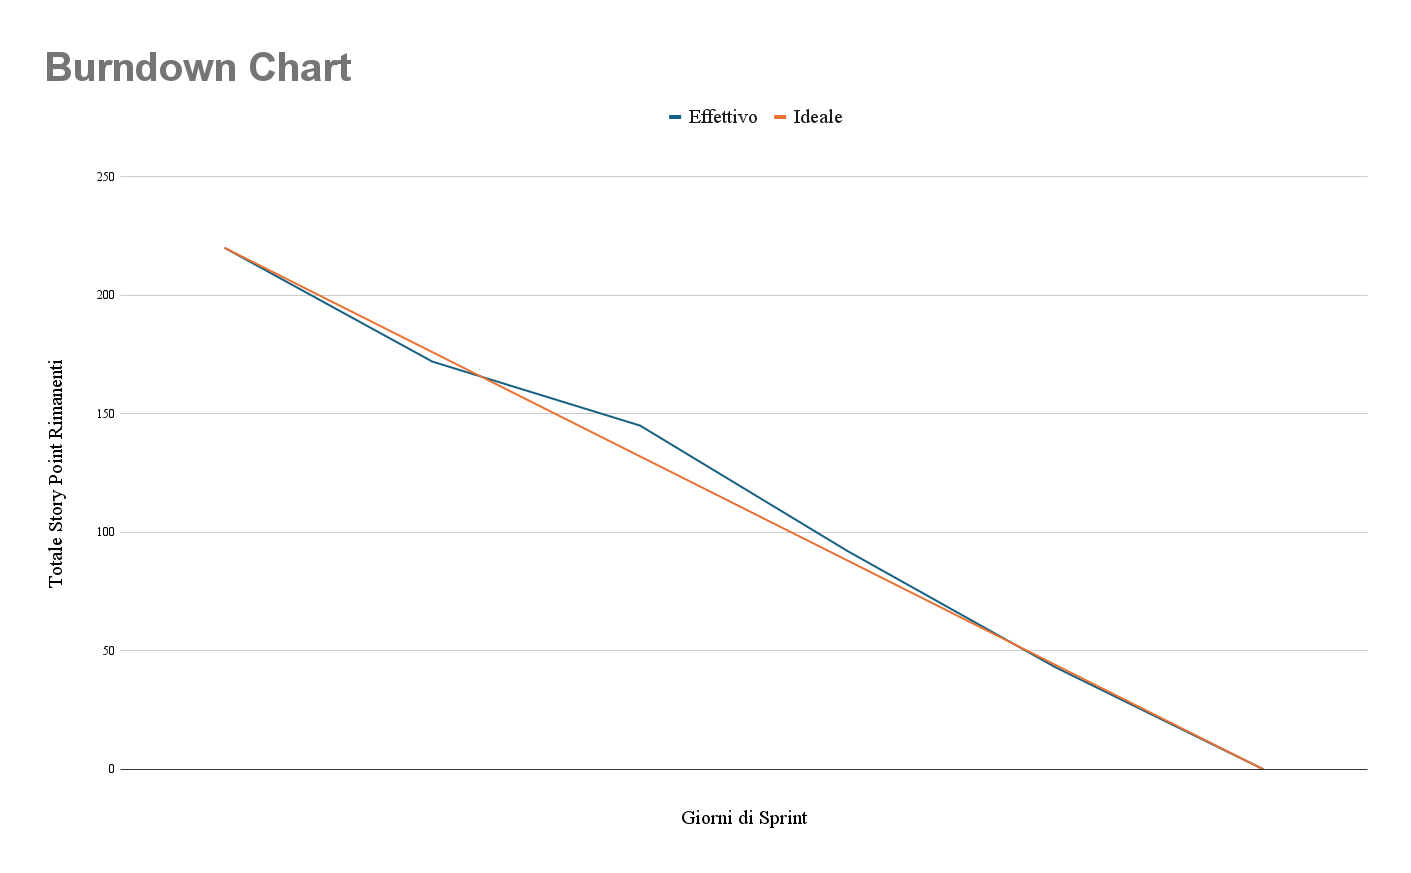
\includegraphics[width=1\linewidth]{D3-G1//Img/BurndownChart.png}
    \caption{L'andamento effettivo non tiene in considerazione le user stories non implementate.}
    \label{fig:enter-label}
\end{figure}

\vspace{12 cm}

\subsection{Test Cases}
È possibile visualizzare i casi di test di EcoTrack al seguente link: \href{https://docs.google.com/spreadsheets/d/19TjIHKf8wvDxEds9eg8yDFcew4lJyGeI82jz5czIyQI/edit?usp=sharing}{EcoTrack - Test Cases}.
\begin{figure}[H]
    \centering
    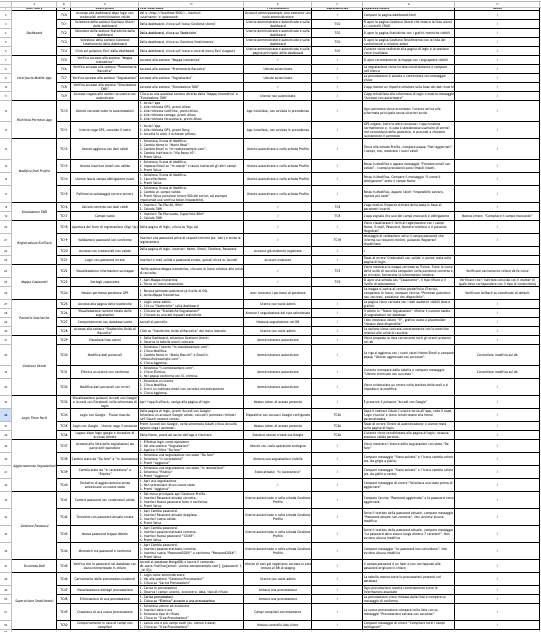
\includegraphics[width=1\linewidth]{D3-G1//Img/Screenshot Test Cases.png}
    \caption{Test Cases Overview}
    \label{fig:enter-label}
\end{figure}

\subsection{Sprint Review}

Durante questa Sprint, il team di sviluppo composto da \textbf{Giulio}, \textbf{Jago} e \textbf{Tommmaso} ha completato diverse user-story fondamentali, lavorando in modo equilibrato su \textit{frontend} e \textit{backend}. Il focus principale dello sprint è stato lo sviluppo delle \textbf{API REST}, l’integrazione con il \textbf{database NoSQL} e la gestione degli \textbf{story points}.

\subsubsection{Obiettivi Sprint Completati}
\begin{enumerate}
  \item Implementazione delle API per la gestione utenti, segnalazioni e smaltimenti.
  \item Connessione tra API e database NoSQL per salvataggio e recupero dati.
  \item Interfacce frontend per:
  \begin{itemize}
    \item Registrazione e Login
    \item Gestione password
    \item Dashboard amministratore
    \item Aggiornamento segnalazioni
  \end{itemize}
  \item Integrazione delle logiche di sicurezza per la protezione dei dati (es. token di accesso).
\end{enumerate}

\subsubsection{Dimostrazione Funzionalità}
Ogni funzionalità completata è stata presentata tramite la \textit{web app} e l’app \textit{mobile}. Le principali azioni dimostrate:
\begin{itemize}
  \item Registrazione utente con messaggio di successo.
  \item Visualizzazione delle unità di raccolta, etichettate tramite segnaposto nella mappa interattiva.
  \item Visualizzazione utenti e gestione dei dati lato amministratore.
\end{itemize}

\subsection{Product Backlog Refinement}
Durante questa fase, il team ha analizzato in dettaglio l’insieme delle user-story presenti nel product backlog, al fine di migliorarne la chiarezza e la pianificazione.

\subsubsection{Scomposizione delle User-Story Complesse}

Alcune user-story sono state identificate come troppo ampie o ambigue per essere realizzate all’interno di uno sprint. Sono state quindi suddivise in sotto-user-story più granulari. \\ Ad esempio la user-story \textit{Notifica Pre-Raccolta} è stata scomposta in \textit{Gestione Preferenze Utente}, \textit{Scheduling delle Notifiche} e \textit{Invio Push lato Mobile}

\subsubsection{Revisione degli Story Points}

Sono stati aggiornati alcuni valori di stima, alla luce di una maggiore comprensione della complessità tecnica:

\begin{itemize}
  \item \textbf{Pannello Statistiche}: Da 5 a 8 story points
  \item \textbf{Login Terze Parti}: Da 5 a 3 story points
  \item \textbf{Saturazione Raccolta}: Da 3 a 5 story points
  \item \textbf{Notifica Pre-Raccolta}: Da 2 a 3 story points
\end{itemize}

\subsubsection{Miglioramento dei Criteri di Accettazione}

Alcune user-story sono state chiarite con criteri di accettazione più specifici e misurabili. Ad esempio:
\begin{itemize}
  \item \textbf{Modifica Dati Profilo}: salvataggio in tempo reale, messaggio di conferma, gestione errori.
  \item \textbf{Visualizzazione Pulizia}: filtro per zona e data, aggiornamenti in tempo reale.
\end{itemize}

\subsubsection{Risultati del Refinement}
Il backlog risulta ora composto da user-story più chiare e attuabili, organizzato con stime più realistiche. quindi pronto per una selezione efficace durante gli sprint planning successivi.


\subsection{Sprint Retrospective}

La maggior parte delle user-story pianificate per lo sprint sono state completate, mentre alcune risultano ancora parzialmente implementate. Il team è riuscito a mantenere un buon ritmo di lavoro costante per tutta la durata dello sprint, ma ha riscontrato alcune difficoltà nella gestione delle tempistiche, specialmente nella fase di integrazione tra report e codice. \\ Questo ha richiesto un riadattamento degli story points nelle ultime giornate di sviluppo. Nonostante le criticità, la collaborazione tra i membri è stata efficace, ciascun componente ha contribuito attivamente sia sul fronte backend che frontend, adottando un approccio di revisione reciproca del codice.

\subsubsection{Punti di Forza}
Durante la Sprint si sono riscontrati diversi elementi positivi che hanno contribuito al buon andamento delle attività:
\begin{itemize}[leftmargin=1.5em]
    \item La \textbf{collaborazione tra i membri del team} è stata efficace, grazie anche alla regolarità delle daily meeting.
    \item Gli obiettivi di Sprint sono stati \textbf{chiaramente definiti} e condivisi, permettendo a ciascun membro di lavorare in modo mirato.
    \item La funzionalità di \textbf{registrazione utenti} è stata completata senza particolari intoppi, risultando stabile e pronta all’uso.
\end{itemize}

\subsubsection{Criticità Riscontrate}
Sono emerse alcune problematiche che hanno influito, in parte, sull'efficienza complessiva:
\begin{itemize}[leftmargin=1.5em]
    \item La parte relativa alla visualizzazione del calendario di \textbf{pulizia stradale} è rimasta \textbf{incompleta}, a causa di difficoltà tecniche legate alle API esterne.
    \item Alcune attività sono risultate \textbf{sottostimate in termini di effort}, generando ritardi e riassegnazioni.
\end{itemize}

\subsubsection{Valutazione Conclusiva dello Sprint}
Lo sprint appena conclusa ha evidenziato una buona maturità del team nella gestione delle funzionalità core, ma anche la necessità di consolidare alcune pratiche legate alla pianificazione e al testing. Le azioni individuate mirano a migliorare la prevedibilità e la qualità del processo, in vista delle successive fasi del progetto \textit{EcoTrack}.
